% !TEX root=../master.tex
\chapter{Multiple Target Tracking}
\label{ch:target_tracking}

% - new for fixed wing / gimbal

Both the tracking UAV and the Handoff UAV track the ground targets using the R-RANSAC-based visual multiple target tracking (VMTT), originally presented in \cite{NiedfeldtBeard13} and \cite{Ingersoll15}. Although there have been many subsequent publications extending and improving the original algorithm
%% ST: Which references are best to include?
(\cite{DeFranco15}, \cite{IngersollNiedfeldtBeard__},
\cite{IngersollNiedfeldtBeard15}, \cite{NiedfeldtIngersollBeard17}),
this is the first work where the algorithm is used extensively on a fixed-wing aircraft. 
Fixed-wing aircraft operate under different conditions and constraints than multi-rotor aircraft. They must maintain forward velocity with non-holonomic motion constraints, and they often fly at higher altitudes and faster speeds. 
These differences require some unique integration and adaptation of the original algorithm into our particular system. 
This chapter will provide a brief overview of the visual frontend and the R-RANSAC algorithm, along with an explanation of both our implementation and results of using R-RANSAC on a fixed-wing vehicle.

\section{Visual Frontend}
\begin{figure}[hbt]
  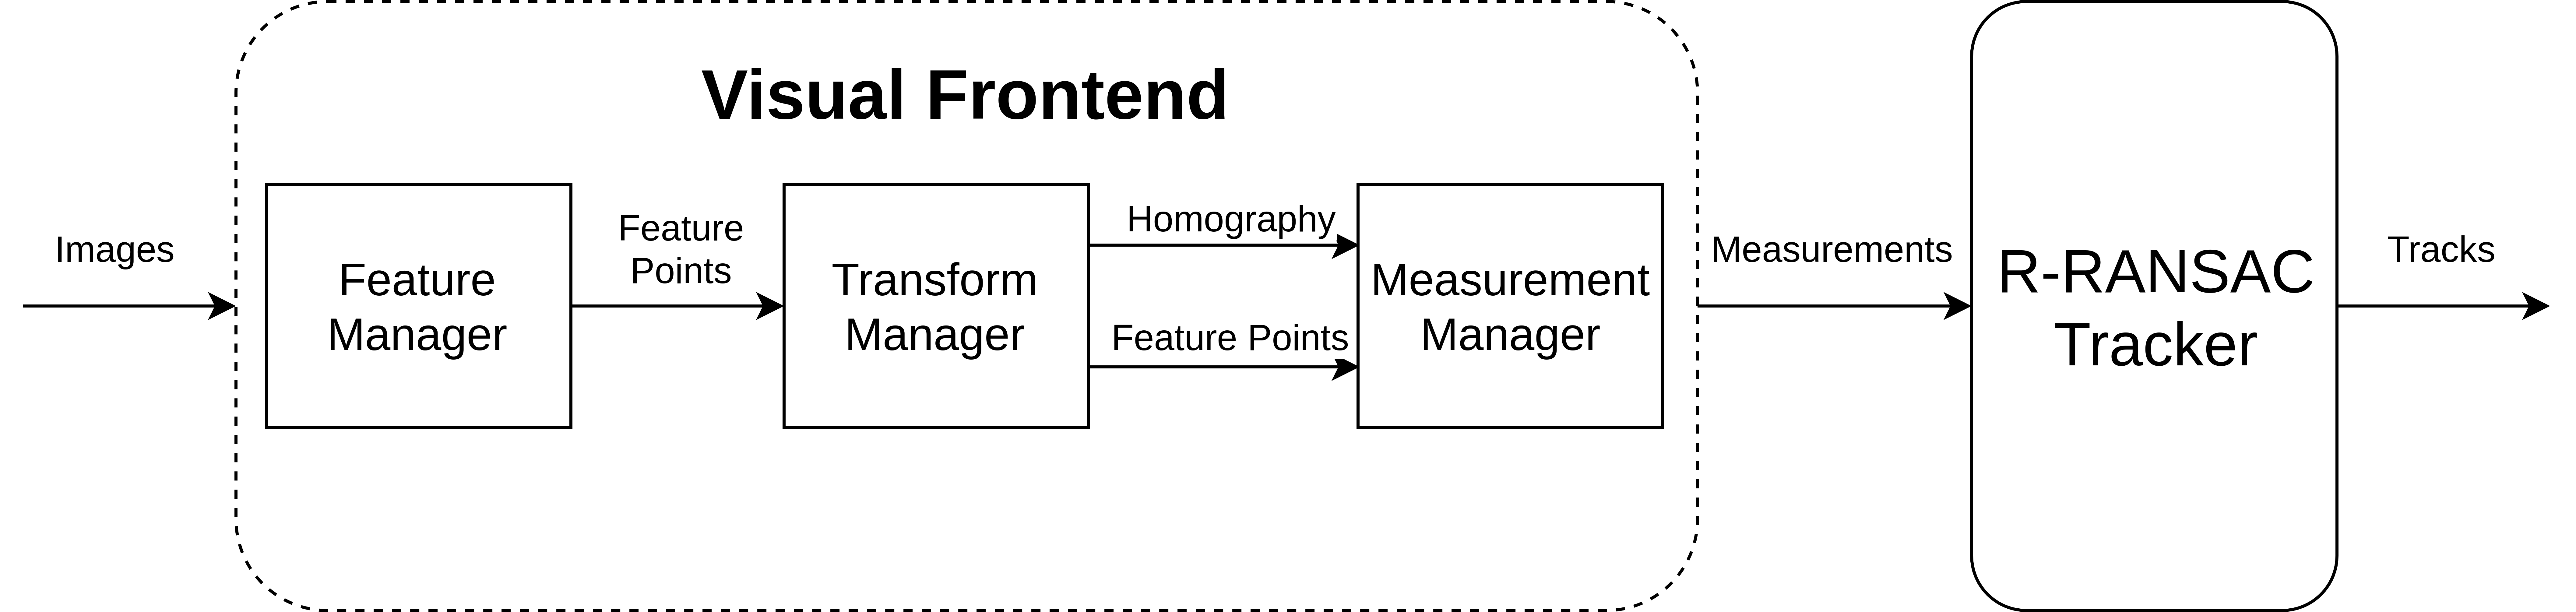
\includegraphics[width=\columnwidth]{figures/vmtt_diagram}
  \caption{Block diagram of visual frontend and R-RANSAC information flow.}
  \label{fig:vmtt_block}
\end{figure}
The visual frontend pipeline is made up of three main blocks--the feature manager, the transform manager, and the measurement manager as seen in Figure~\ref{fig:vmtt_block}. The feature manager receives the current frame as input and finds good features in the image. The features are passed to the transform manager, which estimates the homography between the previous and current frames. The measurement manager uses the image, the features, and the homography to produce meaningful measurements as candidates for new models to track. These measurements are used as input to the R-RANSAC algorithm.

\section{R-RANSAC Tracker}
\subsection{RANSAC Algorithm}
Recursive RANSAC is based upon the original RANSAC (random sample consensus) algorithm, which was first intruduced in \cite{FischlerBolles81}. 
RANSAC is commonly used to fit data to a given model and reject outliers to that model. 
The algorithm uses an iterative process to determine the best model parameters to describe the largest subset of the data possible. 
On each iteration, a subset of the data is randomly sampled containing the minimum number of data points required to represent the model. 
Using the selected points, the appropriate model parameters are computed, and the remaining points are classified as inliers or outliers to the proposed model based on some predetermined error threshold. All points that lie withing the error threshold are referred to as the consensus set. 
If the consensus set has a sufficient number of points, the model parameters are recomputed using all of the points in the consensus set. 
The points outside the consensus set are considered outliers and have no influence on the resulting model. This process is repeated a fixed number of times and the model with the largest consensus set is considered to be the best model and is used as the final solution. 
% Potentially add a linear example 

By way of example, consider that we wanted to use RANSAC to perform linear regression on a set of points. The model would be a straight line and the model parameters could be the slope and y-intercept of the line. The minimum number of points required to define a line is two, so in each iteration of the algorithm, the random sample would consist of two points. Using these two points, we would form a line and determine which points lie within some distance threshold of that line. If the consensus set was sufficiently large, we would consider the line to be a good model for the data and recompute the best fit line using only the points within the consensus set. This process would be repeated for the desired number of iterations, saving the model with the largest consensus set as the best model for the data. Using RANSAC to estimate model parameters in this way has the added advantage of being able to identify and completely reject outliers or exessively noisy datapoints, allowing the model to be more accurate and more representative of the true data.

In the R-RANSAC algorithm, the models are motion models through time. We typically use constant acceleration or constant jerk linear motion models to describe the motion of objects. R-RANSAC uses RANSAC to find and initialize good models, which are then "recursively" propagated through time using a linear filter. RANSAC is then applied to all measurements which do not belong to a model that is currently being tracked to determine if there are good models among the remaining outliers. This allows the R-RANSAC tracker to simultaneously manage an arbitrary number of tracks at any given time.

\section{Adaptations for Fixed-wing vehicles}
\subsection{Two-axis gimbal}
One of the main differences between tracking from a fixed-wing vehicle as opposed to a multirotor, is that the vehicle must remain in constant motion. Accordingly, a gimbal is necessary to maximize the aircraft's ability to maintain a line of sight to the target. We chose to use a two-axis gimbal for this project to allow control of both the azimuth and elevation angles of the camera. The appropriate azimuth and elevation angles are computed according to
\begin{equation}
  \az = \atantwo(\los_y, \los_x)\;,
\end{equation}
and
\begin{equation}
  \el = -\asin(\los_z)\;,
\end{equation}
where $\los$ is the normalized line of sight vector from the UAV to the target in the vehicle body frame.
%% ST: ADD MORE HERE?

\subsection{Parameter Tuning}
Some of the other challenges of implementing the R-RANSAC tracker on a fixed-wing vehicle include higher operating altitudes, faster velocities, and continuously varying viewpoints of the target.
These conditions can make it more difficult for the vehicle to pick up on good, consistent features of the target and can also lead to high variation in the apparent motion of the target.
The apparent motion of the target in the camera frame is minimized when the line of sight to the target and the target's velocity are nearly aligned.
In a constant orbit about a ground target with nearly constant velocity, this alignment happens twice per revolution.
R-RANSAC assumes that targets of interest are moving and therefore uses motion in the image plane to track targets, which makes it more difficult for the tracker to continue tracking the target when the apparent motion is low.

To overcome these challenges, we tuned the algorithm parameters to help the tracker be better suited to having fewer good features and periodically low apparent motion. Table~\ref{tab:vmtt_params} summarizes our parameter choices for the tracking algorithm.

% Please add the following required packages to your document preamble:
% \usepackage[table,xcdraw]{xcolor}
% If you use beamer only pass "xcolor=table" option, i.e. \documentclass[xcolor=table]{beamer}
% Please add the following required packages to your document preamble:
% \usepackage{graphicx}
% \usepackage[table,xcdraw]{xcolor}
% If you use beamer only pass "xcolor=table" option, i.e. \documentclass[xcolor=table]{beamer}
\begin{table}[hbt]
\caption{R-RANSAC Tracking Parameters}
\label{tab:vmtt_params}
\centering
\resizebox{\columnwidth}{!}{%
\begin{tabular}{|>{\centering\arraybackslash}m{0.15\columnwidth}|>{\centering\arraybackslash}m{0.27\columnwidth}|>{\centering\arraybackslash}m{0.09\columnwidth}|>{\centering\arraybackslash}m{0.09\columnwidth}|>{\centering\arraybackslash}m{0.3\columnwidth}|}
\hline
\textbf{Param}                      & \textbf{Description}                                                          & \textbf{Default} & \textbf{Ours} & \textbf{Reasoning}                                                                          \\ \hline
frame stride               & Number of frames between measurements                                                  & 2       & 3         & More frames between measurements equates to more motion.                           \\ \hline
minimum feature velocity   & minimum allowable feature velocity                                                     & 0.002   & 0.0005    & Allows the tracker to detect slower tracks                                         \\ \hline
Nw                         & Window/history size                                                                    & 10      & 25        & A longer window allows the tracker to better determine which tracks are persistent \\ \hline
M                          & Maximum number of models                                                               & 30      & 10        & Allows for fewer good models; less likely to pick up on noise                      \\ \hline
tauR                       & Inlier region threshold                                                                & 0.07    & 0.045     & Better suited for smaller targets                                                  \\ \hline
tau\_CMD                   & consecutive missed detections (CMD) threshold                                          & 4       & 10        & Allows for more missed detections                                                  \\ \hline
tau\_Vmax                  & maximum model speed                                                                    & 0.043   & 0.025     & Allows for slower moving targets                                                   \\ \hline
tau\_T                     & Tracks must have a lifetime counter above this threshold to be considered good tracks. & 4       & 25        & Requires tracks to persist for longer before being considered a good model         \\ \hline
\end{tabular}%
}
\end{table}

\section{Results}
Using the R-RANSAC tracker and a two-axis gimbal setup, we were able to achieve reasonable tracking results for moving ground targets. We tested the tracking algorithm on a fixed-wing aircraft flying approximately 300 meters above a moving vehicle on the ground. With proper tuning, we were able to get the UAV to track the vehicle despite significant jitter in camera feed. Figure~\ref{fig:afrl_tracking} shows a snapshot of tracking the moving ground target.

\begin{figure}[hbt]
  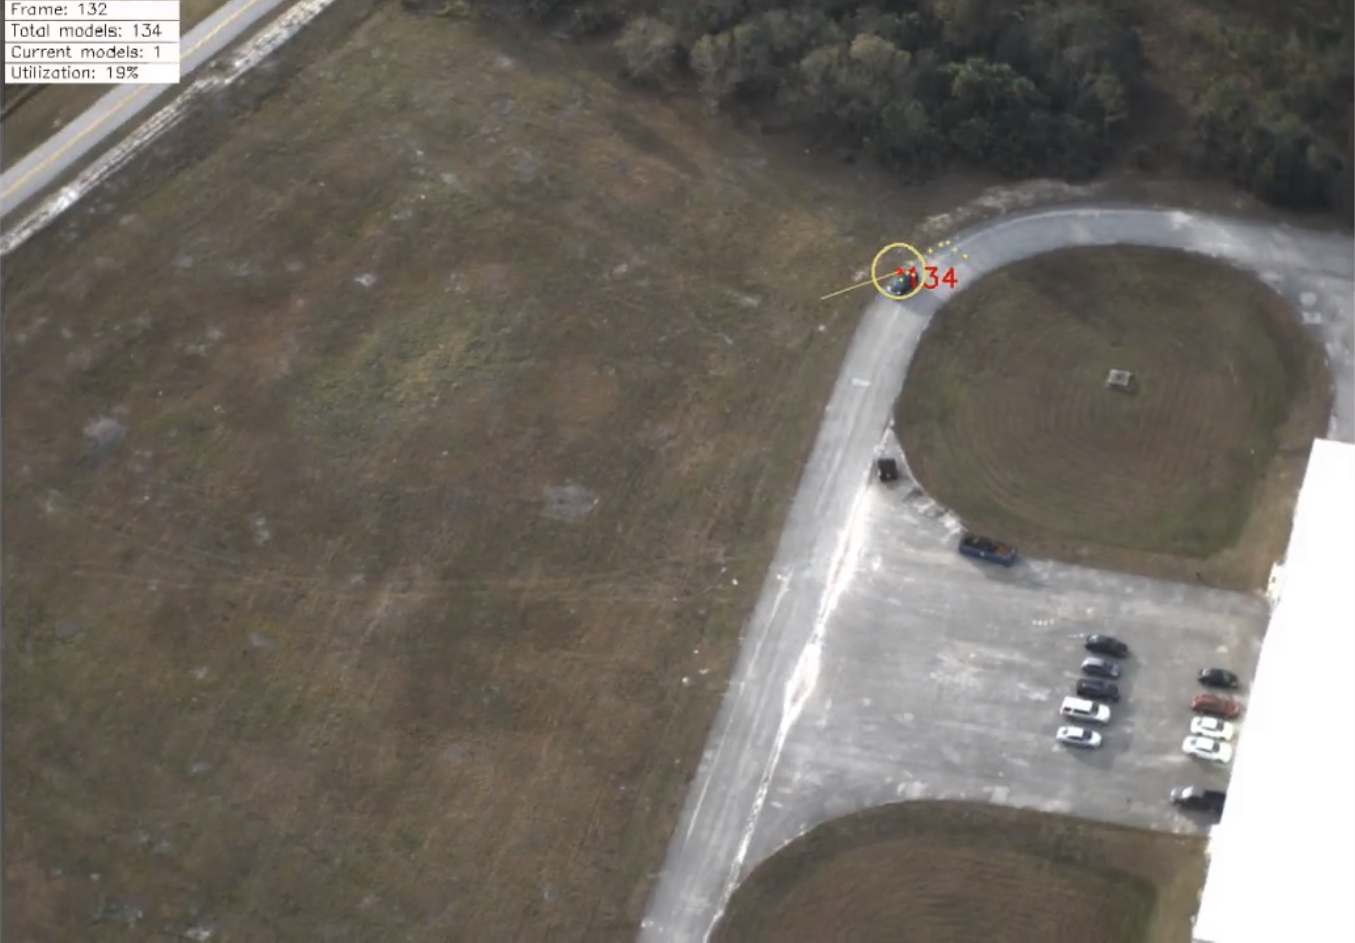
\includegraphics[width=\columnwidth]{figures/afrl_tracking}
  \caption{Snapshot of tracking a moving ground target from a fixed-wing aircraft}
  \label{fig:afrl_tracking}
\end{figure}
